
\documentclass{sigplanconf}

% The following \documentclass options may be useful:

% preprint      Remove this option only once the paper is in final form.
% 10pt          To set in 10-point type instead of 9-point.
% 11pt          To set in 11-point type instead of 9-point.
% authoryear    To obtain author/year citation style instead of numeric.

\usepackage[dvipsnames]{xcolor}
\usepackage{siunitx}
\usepackage{amsmath}
\usepackage{amsfonts}
\usepackage{amssymb}
\usepackage{array}
\newcolumntype{L}[1]{>{\raggedright\let\newline\\\arraybackslash\hspace{0pt}}m{#1}}
\newcolumntype{C}[1]{>{\centering\let\newline\\\arraybackslash\hspace{0pt}}m{#1}}
\newcolumntype{R}[1]{>{\raggedleft\let\newline\\\arraybackslash\hspace{0pt}}m{#1}}
\usepackage[utf8]{inputenc}
\usepackage[english]{babel}
\usepackage{pgfplots}
\usepackage{url}
\usepackage{hyperref} 
\usepackage{float}
\usepackage{tabularx,caption}
\usepackage{csvsimple}
\usepackage{listings,mdframed}


\lstset{
	language=c,
	keywordstyle=\bfseries\ttfamily\color[rgb]{0,0,1},
	identifierstyle=\ttfamily,
	commentstyle=\color[rgb]{0.133,0.545,0.133},
	stringstyle=\ttfamily\color[rgb]{0.627,0.126,0.941},
	showstringspaces=false,
	basicstyle=\tiny,
numberstyle=\tiny,
numbers=right,
	stepnumber=1,
	numbersep=10pt,
	tabsize=1,
	breaklines=true,
	prebreak = \raisebox{0ex}[0ex][0ex]{\ensuremath{\hookleftarrow}},
	breakatwhitespace=false,
	aboveskip={1.5\baselineskip},
  columns=fixed,
  upquote=true,
  extendedchars=true,
 frame=single,
 inputencoding=utf8,
    literate={á}{{\'a}}1 {ã}{{\~a}}1 {â}{{\~a}}1 {é}{{\'e}}1 {ê}{{\'e}}1 {ç}{{\'c}}1 {ú}{{\'u}}1 {ó}{{\'o}}1 {í}{{\'i}}1,
 %backgroundcolor=\color{lbcolor},
}


\hypersetup{colorlinks =false}

\begin{document}

\special{papersize=8.5in,11in}
\setlength{\pdfpageheight}{\paperheight}
\setlength{\pdfpagewidth}{\paperwidth}

\conferenceinfo{CONF 'yy}{Month d--d, 20yy, City, ST, Country} 
\copyrightyear{20yy} 
\copyrightdata{978-1-nnnn-nnnn-n/yy/mm} 
\doi{nnnnnnn.nnnnnnn}

% Uncomment one of the following two, if you are not going for the 
% traditional copyright transfer agreement.

%\exclusivelicense                % ACM gets exclusive license to publish, 
                                  % you retain copyright

%\permissiontopublish             % ACM gets nonexclusive license to publish
                                  % (paid open-access papers, 
                                  % short abstracts)

\titlebanner{banner above paper title}        % These are ignored unless
\preprintfooter{short description of paper}   % 'preprint' option specified.

\title{ Code Profiling and Performance Analysis for Dense Matrix Multiplication Algorithms on Intel\textsuperscript{\textregistered} Core\textsuperscript{TM} i7-3635QM  }

\subtitle{}

\authorinfo{Filipe Costa Oliveira}
           {Universidade do Minho}
           {a57816@alunos.uminho.pt}
           
\authorinfo{Sérgio Manuel Rodrigues Caldas}
           {Universidade do Minho}
           {a57779@alunos.uminho.pt}

\maketitle

\begin{abstract}
In a complex multi-core, multi-processor software developing environment, tracking the performance of the code can be a non-trivial task.\par 
We describe the usage of a visual performance model that has given considerable insight into the performance of the code and helped to trace a optimization time line for future code optimization.\par 
For code instrumentation we used PAPI\cite{papi}, which is a programing interface for accessing hardware performance counters. PAPI events can count floating point operations, cycles, instructions and cache accesses. Triggering PAPI to start/stop counting for each algorithm and process event results is a good understanding of the algorithm performance. \end{abstract}

\section{Hardware characterization}
The platform studied at Search6 is a dual-socket system equipped with two
Intel\textsuperscript{\textregistered} Nehalem processors.
The system, referenced as compute node
431, has two Intel\textsuperscript{\textregistered} Xeon\textsuperscript{\textregistered} E5-5650 (Nehalem architecture) and features 48 GB of DDR3 RAM, supported at a frequency of 1333 MHz divided in 3 memory channels. \par 

The second computing platform, our team laptop, is a  Intel\textsuperscript{\textregistered} Core\textsuperscript{TM} i7-3635QM (Ivy Bridge architecture). The system features 16 GB of DDR3 RAM, supported at a frequency of 1600MHz, divided in 2 memory channels. \par 

The characteristics of the CPUs on the two computing platforms are presented in the table \ref{table:characterization}.

\begin{table}[]
\centering
  \begin{tabular}{ | L{2.6cm} | R{2.2cm} | R{2.3cm} | }
  
    \hline
    System & compute-401 & team laptop \\ \hline \hline
        \# CPUs & 2 & 1 \\ \hline
    CPU & Intel\textsuperscript{\textregistered} Xeon\textsuperscript{\textregistered} X5650 & Intel\textsuperscript{\textregistered} Core\textsuperscript{TM} i7-3635QM \\ \hline 
    Architecture & Nehalem & Ivy Bridge \\ \hline 
    \# Cores per CPU & 6  & 4 \\ \hline 
    \# Threads per CPU & 12 & 8 \\ \hline 
    Clock Freq. & 2.66 GHz & 2.4 GHz \\ \hline \hline 
    L1 Cache & 192KB \newline 32KB per core & 128KB  \newline 32KB per core \\ \hline 
    L2 Cache & 1536KB  \newline  256KB per core  & 1024KB \newline 256KB per core \\ \hline 
    L3 Cache & 12288KB \newline shared & 6144KB \newline  shared  \\ \hline \hline 
    Inst. Set Ext. & SSE4.2 & SSE4.2 \& AVX \\ \hline 
        \#Memory Channels & 3 & 2 \\ \hline \hline

    Vendors Announced Peak Memory BW & 32 GB/s & 25.6 GB/s\\ \hline
    Measured\cite{stream} Peak Memory BW & 25.1GB/s & 15.5 GB/s\\ \hline
  \end{tabular}
     \caption{Architectural characteristics of the two evaluation platforms.}
    %% \label{table:characterization}
\end{table}

\section{Roofline Model for single-precision FP}
The Roofline Model characterizes the system in terms of attainable peak performance relating together floating-point performance, memory performance, and arithmetic intensity in a two dimensional graph. More importantly, it graphically shows the penalty associated with not including certain software optimizations.\par 
With the peak values of the first two metrics a Roofline is drawn, which
is the theoretical limit for the system performance. \par 
The computational intensity was used for measuring the CPU peak
performance, as it considers all types of instructions.\par
Roofline model refers to the maximum memory bandwidth of the system and it was determined using the STREAM benchmark\cite{stream}. As expected the manufacturers advertised Max Memory bandwidth value (in GB/s) was unable to be reached by experimentation.\par 

\subsection{Determining Roofline model ceiling for the team's laptop} 
The peak computational intensity was calculated with the following formula

\[ \#Cores * Frequency * \frac{AVX width}{AVX    troughtput}  \]

The clock frequency and
number of cores were obtained by consulting the Intel\cite{intel_5650}\cite{intel_i7} CPU specifications, while the number of
instructions issued per clock cycle were determined based on number of instructions that can be decoded per clock cycle\cite{intel_intrinsics} and the minimal delay (The time unit used was core clock cycles) generated by instructions in a dependency chain\cite{agner}, of the processors. 
\par 
The value obtained represents the horizontal roof of the model. The tilted roof of the
Roofline model refers to the maximum memory bandwidth of the system and it was determined
using the STREAM benchmark\cite{stream}. These values and measurement conditions are presented in Apendix \ref{appendix:stream}.

\subsection{Determining additional Roofline ceilings for team's laptop} 
Additional ceilings were added, defining possible performance subtractors. The ceilings for the team's test laptop, and their importance, are presented below:

\subsubsection{Multiplication / Add Balance}
Ivy Bridge processors have separate multipliers and adders on each core. For taking full advantage of the functional units, the algorithm must have an approximate number of multiplications and additions. If that equality is not ensured performance is decreased at least to half.

\subsubsection{AVX}
In single precision, AVX represents one operation can contain 8 single precision floats. 
Without AVX vectorization only 1/8 of the peak performance is achievable.

\subsubsection{Instruction Level Parallelism}
If independent instructions are kept in the pipeline without instruction level parallelism, performance will fall. Even the simplest arithmetic operation takes more than 1 clock cycle to compute\cite{agner}. If no instruction level parallelism is ensured, we would consequently have idle functional units, resulting in a performance decrease by at least to half. Note that, despite a decrease to half seem a large performance withhold, it could be exponentially worsened if we consider the delay generated by instruction like single precision float division.

\subsubsection{Thread Level Paralelism}
Thread Level Parallelism allows the usage of all available cores in the CPU. If only one core is used in our algorithm, the maximum performance would be limited by a factor of 4 -- the number of cores of Intel\textsuperscript{\textregistered} Core\textsuperscript{TM} i7-3635QM.

\subsection{Ordering ceilings according to Matrix Multiplication}

If we want to compute A*B = C where A, B and C are matrices of size $N * N$ it would require $N^{3}$ arithmetic operations.Those arithmetic operations are equally divided in sums and products. For most of the kernels achieving this equality between multiplication and additions is very difficult to achieve. In our kernel it is almost implied, and should be our first ceiling.
\par  The second and easiest to implement optimization, would be instruction level parallelism. ILP is also the most likely optimization to be implemented automatically by the compiler.\par
Since without AVX vectorization only 1/8 of the peak performance is achievable that should be the next ceiling of the matrix multiplication roofline for  i7-3635QM.\par 
The last, and most difficult to implement optimization is Thread Level Parallelism. Without it the peak performance its reduce by a factor of 4.

\subsection{Obtained Roofline Model on Team Laptop}

Figure \ref{figure:roofline_team}
illustrates the Roofline Model for Intel\textsuperscript{\textregistered} Core\textsuperscript{TM} i7-3635QM present on the team's laptop.\\\par 

\begin{figure}[H]
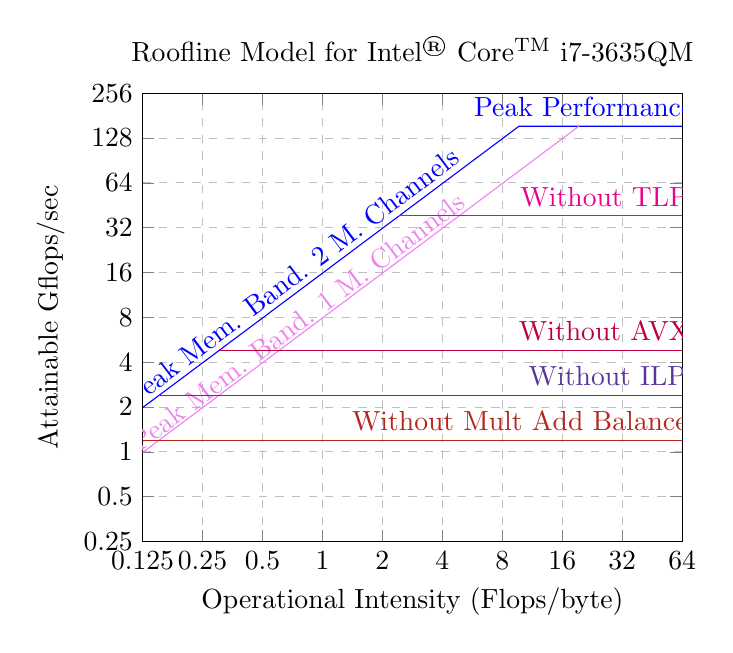
\begin{tikzpicture}
\begin{axis}[
    title={Roofline Model for Intel\textsuperscript{\textregistered} Core\textsuperscript{TM} i7-3635QM},
    xlabel={Operational Intensity (Flops/byte)},
    ylabel={Attainable Gflops/sec},
    xmin=0.125, xmax=64,
    ymin=0.25, ymax=256,
    xtick={0.125,0.25,0.5,1,2,4,8,16,32,64},
    ytick={0.25,0.5,1,2,4,8,16,32,64,128,256},
    legend pos=north west,
    ymajorgrids=true,
    xmajorgrids=true,
    grid style=dashed,
    xmode=log,
    ymode=log,
    log ticks with fixed point
]
 
\addplot[
    color=blue,
    ]
    coordinates {
    (0.125,1.9805)(9.695,153.6)(64,153.6)
    };
    \node[rotate=37,text=blue] at (axis cs: 0.70,15) {Peak Mem. Band. 2 M. Channels};
    
\addplot[
    color=Violet,
    ]
    coordinates {
    (0.125,0.99025)(19.389,153.6)
    };
    \node[rotate=37, text=Violet] at (axis cs: 0.75,7.5) {Peak Mem. Band. 1 M. Channels};    
    
\node [above,text=blue] at (axis cs: 20.5,153.6) {Peak Performance};
    




    
\addplot[
    color=BrickRed,
    ]
    coordinates{
    (0.07575,1.2)(64,1.2)
    };
\node [above,text=BrickRed] at (axis cs: 10.7,1.2) { Without Mult Add Balanced};

\addplot[
    color=purple,
    ]
    coordinates{
    (0.303,4.8)(64,4.8)
    };
    
\node [above,text=purple] at (axis cs: 26,4.8) { Without AVX };

\addplot[
    color=RoyalPurple,
    ]
    coordinates {
    (0.151,2.4)(64,2.4)
    };
    
\node [above, text=RoyalPurple] at (axis cs: 27,2.4) { Without ILP };

\addplot[
    color=magenta,
    ]
    coordinates {
    (2.42,38.4)(64,38.4)
    };
    
\node [above, text=magenta] at (axis cs: 26,38.4) { Without TLP };



\end{axis}
\end{tikzpicture}
\caption{Roofline Model for Team Laptop}
\label{figure:roofline_team}
\end{figure}

\subsection{Obtained Roofline Model on Search6 Node}
Figure \ref{figure:roofline_search}
illustrates the Roofline Model for Intel\textsuperscript{\textregistered} Xeon\textsuperscript{\textregistered} X5650 present on the Search6 Node.\\\par 

\begin{figure}[H]
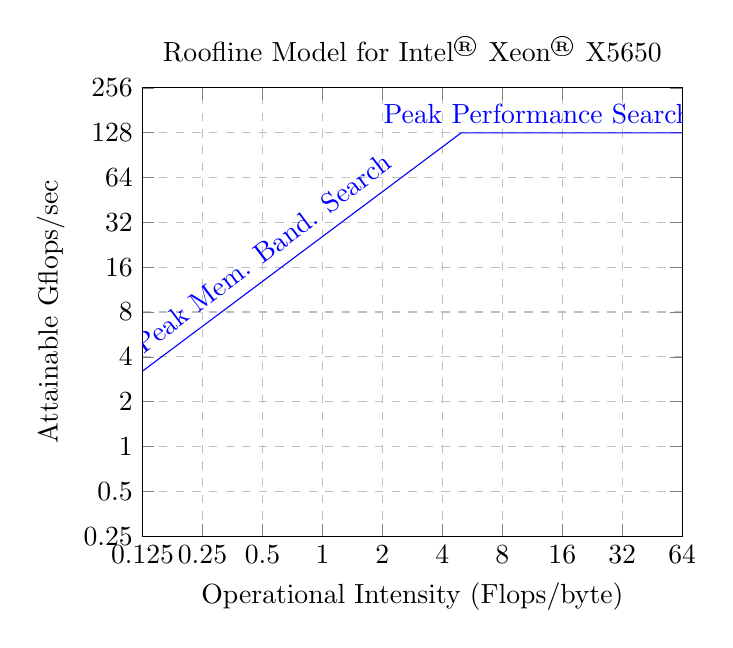
\begin{tikzpicture}
\begin{axis}[
    title={Roofline Model for Intel\textsuperscript{\textregistered} Xeon\textsuperscript{\textregistered} X5650},
    xlabel={Operational Intensity (Flops/byte)},
    ylabel={Attainable Gflops/sec},
    xmin=0.125, xmax=64,
    ymin=0.25, ymax=256,
    xtick={0.125,0.25,0.5,1,2,4,8,16,32,64},
    ytick={0.25,0.5,1,2,4,8,16,32,64,128,256},
    legend pos=north west,
    ymajorgrids=true,
    xmajorgrids=true,
    grid style=dashed,
    xmode=log,
    ymode=log,
    log ticks with fixed point
]
 
\addplot[
    color=blue,
    ]
    coordinates {
    (0.125,3.2088)(4.974,127.68)(8,127.68)(16,127.68)(32,127.68)(64,127.68)
    };
    \node[rotate=37, text=blue] at (axis cs: 0.5,20) {Peak Mem. Band. Search};

\node [above,text=blue] at (axis cs: 12,127.68) {Peak Performance Search};
\end{axis}
\end{tikzpicture}
\caption{Roofline Model on Search Node}
\label{figure:roofline_search}
\end{figure}

\subsection{Roofline Model Team Laptop vs Roofline Model Search}

\begin{figure}[H]
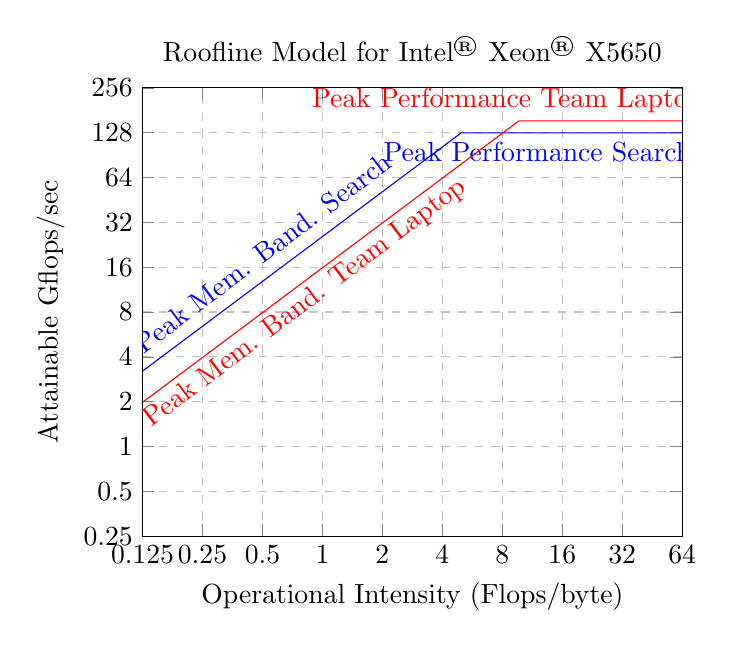
\begin{tikzpicture}
\begin{axis}[
    title={Roofline Model for Intel\textsuperscript{\textregistered} Xeon\textsuperscript{\textregistered} X5650},
    xlabel={Operational Intensity (Flops/byte)},
    ylabel={Attainable Gflops/sec},
    xmin=0.125, xmax=64,
    ymin=0.25, ymax=256,
    xtick={0.125,0.25,0.5,1,2,4,8,16,32,64},
    ytick={0.25,0.5,1,2,4,8,16,32,64,128,256},
    legend pos=north west,
    ymajorgrids=true,
    xmajorgrids=true,
    grid style=dashed,
    xmode=log,
    ymode=log,
    log ticks with fixed point
]

\addplot[
    color=blue,
    ]
    coordinates {
    (0.125,3.2088)(4.974,127.68)(8,127.68)(16,127.68)(32,127.68)(64,127.68)
    };
    \node[rotate=37, text=blue] at (axis cs: 0.5,20) {Peak Mem. Band. Search};

\node [below,text=blue] at (axis cs: 12,127.68) {Peak Performance Search};

\addplot[
    color=red,
    ]
    coordinates {
    (0.125,1.9805)(9.695,153.6)(64,153.6)
    };
    \node[below,rotate=37,text=red] at (axis cs: 0.70,12) {Peak Mem. Band. Team Laptop};
    
    
\node [above,text=red] at (axis cs: 8.5,148.6) {Peak Performance Team Laptop};

\end{axis}
\end{tikzpicture}
\caption{Roofline Model Team Laptop vs Roofline Model Search}
\label{figure:roofline-search-team}
\end{figure}

\section{Metrics for good performance and time measurement}

The performance of each application can be characterized by the rate of algebraic computation, the number of instructions per cycle and the number of memory loads per cycle. From those three rates we can infer potential bootlenecks.\par 

\subsection{Counters for floating point operations}
The rate of algebraic computation, expressed as \textbf{ Flops Per Cycle}, can be estimated based on PAPI following events\par 


\begin{table}[H]
\centering
  \begin{tabular}{ | L{2.5cm} | R{5cm} |  }
      \hline
Name& Description \\
    \hline
PAPI\_FP\_OPS & Floating point operations          \\                   
PAPI\_SP\_OPS & Floating point operations  optimized to count scaled single precision vector operations            \\        
PAPI\_DP\_OPS & Floating point operations  optimized to count scaled double precision vector operations            \\        
PAPI\_VEC\_SP & Single precision vector/SIMD instructions    \\                        
PAPI\_VEC\_DP & Double precision vector/SIMD \\
    \hline

\end{tabular}
\caption{Counters  used  for  measuring  floating  point  operations.}
\label{table:table_fp_ops}
\end{table}

Table \ref{table:table_fp_ops} lists
the  counters  used  for  measuring  floating  point  operations. Of those only the operations including single precision floats are of interest in our case study.\par 

 For  vector  instructions,
the measured values have to be multiplied by the corresponding  vector  length.  \par 
Thus,  the  total  number  of  single precision  floating
point operations on a Ivy Bridge micro-architecture is given by



\subsection{Counters for memory traffic}
\begin{table}[H]
\centering
  \begin{tabular}{ | L{2.5cm} | R{5cm} |  }
      \hline
Name& Description \\
    \hline
    
    PAPI\_L3\_TCR & Level 3 total cache reads      \\                     
PAPI\_L3\_TCW &  Level 3 total cache writes     \\  

PAPI\_L2\_TCM &  Level 2 cache misses       \\                    
PAPI\_L3\_TCM &  Level 3 cache misses    \\   

PAPI\_L2\_TCA & Level 2 total cache accesses    \\                       
PAPI\_L3\_TCA &  Level 3 total cache accesses   \\  
PAPI\_LD\_INS &  Load instructions   \\ 
PAPI\_SR\_INS &  Store instructions   \\  



    \hline

\end{tabular}
\caption{Counters  used  for  memory traffic calculations.}
\label{table:table_mem}
\end{table}

Table \ref{table:table_mem} lists
the  counters  used  for  measuring  memory traffic.
Thus,  in order to compute the arithmetic intensity we will use
\begin{equation}
  \frac{\text{computed value for floating point operations} }{{\text{PAPI\_LD\_INS}}+\text{PAPI\_SR\_INS}}
\end{equation}



\par 
\subsubsection{Measurement limitations}
Despite L1 total cache access being stated as available by PAPI tool, we were unable to produce any measurement regarding that metric.
\par 
For our cpu micro-architecture and our kernel and library version we were unable to measure single and double precision metrics operations at the same experiment due to hardware counters limitation. For our case study that caveat did not inferred validity limitations in our calculations and predictions.


\subsubsection{Relating Memory Counters with potential memory bottlenecks}
L1 (PAPI\_L1\_TCM), L2 (PAPI\_L2\_TCM), and L3 (PAPI\_L3\_TCM) cache miss ration provides insight into suspected memory bottlenecks. In order to infer potential bottlenecks we must analyse the variance of those 3 miss values for different size inputs. Based on that variation we can predict if the application will likely suffer from significant L3 and DRAM scalability problems. \par We must give more importance to the L3 Cache miss counters since L3 cache misses directly translate into off-chip bandwidth, with the consequence of the time penalty associated to it being wider.\par 
\subsection{Counters for timing}
Time measurement (expressed in $\mu$s) for kernel execution was acquired using PAPI\_TIMERS. The used function (PAPI\_get\_real\_usec()) always succeeds (error-free) since it is guaranteed to exist on every PAPI supported platform.



\section{Operational intensity study of dense matrix multiplication algorithms}

In our case study we use the example of matrix-matrix multiplication to illustrate issues that arise when developing kernels requiring large data sets. 
\par In particular, we consider the problem of developing a kernel to compute C = A.B , where A , B , and C are dense matrices of size N * N, each represented as 2-dimensional array in our kernel. Matrix A has \textbf{i} index for row access and \textbf{k} index for column access.
Matrix B has \textbf{k} index for row access and \textbf{j} index for column access. Matrix C has \textbf{i} index for row access and \textbf{j} index for column access.\par 
We first specify the experimental setup; Then
we discuss the various experiments. \par 
We will also analyse the nested loops order for the indexes i,j,k and its affectance in overall kernel performance.

\subsection{Experimental  setup}
We  ran  all  experiments  on  the  platform described earlier as team laptop, for one operating system. Appendix \ref{appendix:papi_avail} describes library versions, the operation system and platform relevant information.PAPI libraries and the developed kernels were compiled using gcc v.4.9.3, with  flags  ”-std=c99  -lpapi”, for non vectorized kernel measurements, and with flags "-O3 -ftree-vectorize -std=c99 -lpapi". \par 
The
data  reported  in  the  plots  is  always  the 3-best  of 
8 repetitions,  with 5\% tolerance. \par 

\subsubsection{Different dataSet sizes}
To investigate the kernel behavior and predict performance bottlenecks, for the developed experimental kernels, different dataset sizes were chosen in order to propitiate 4 distinct situations:
\begin{enumerate}
\item data set completely fitted in L1 cache; Each Matrix has a size of 48 -- resulting in a total data set size of 27KB.
\item dataset completely fitted in L2 cache;  Each Matrix has a size of 128 -- resulting in a total dataset size of 196KB. 
\item data set completely fitted in L3 cache; Each Matrix has a size of 512 -- resulting in a total dataset size of  3072KB.
\item data set completely fitted in Main memory; Each Matrix has a size of 2048 -- resulting in a total dataset size of 49152KB.
\end{enumerate}

\subsection{Nested Loops for single threaded dot ijk}

Given the defined matrices and their size, considering the loop order ijk, we compute their product based on the function in the appendix \ref{appendix:mm_ijk.c}.

For the specific nested loops order, Matrix A is accessed row major, Matrix B is accessed column major, and Matrix C is accessed row major, as described in figure \ref{figure:loop_ijk}.

\begin{figure}[H]
\centering
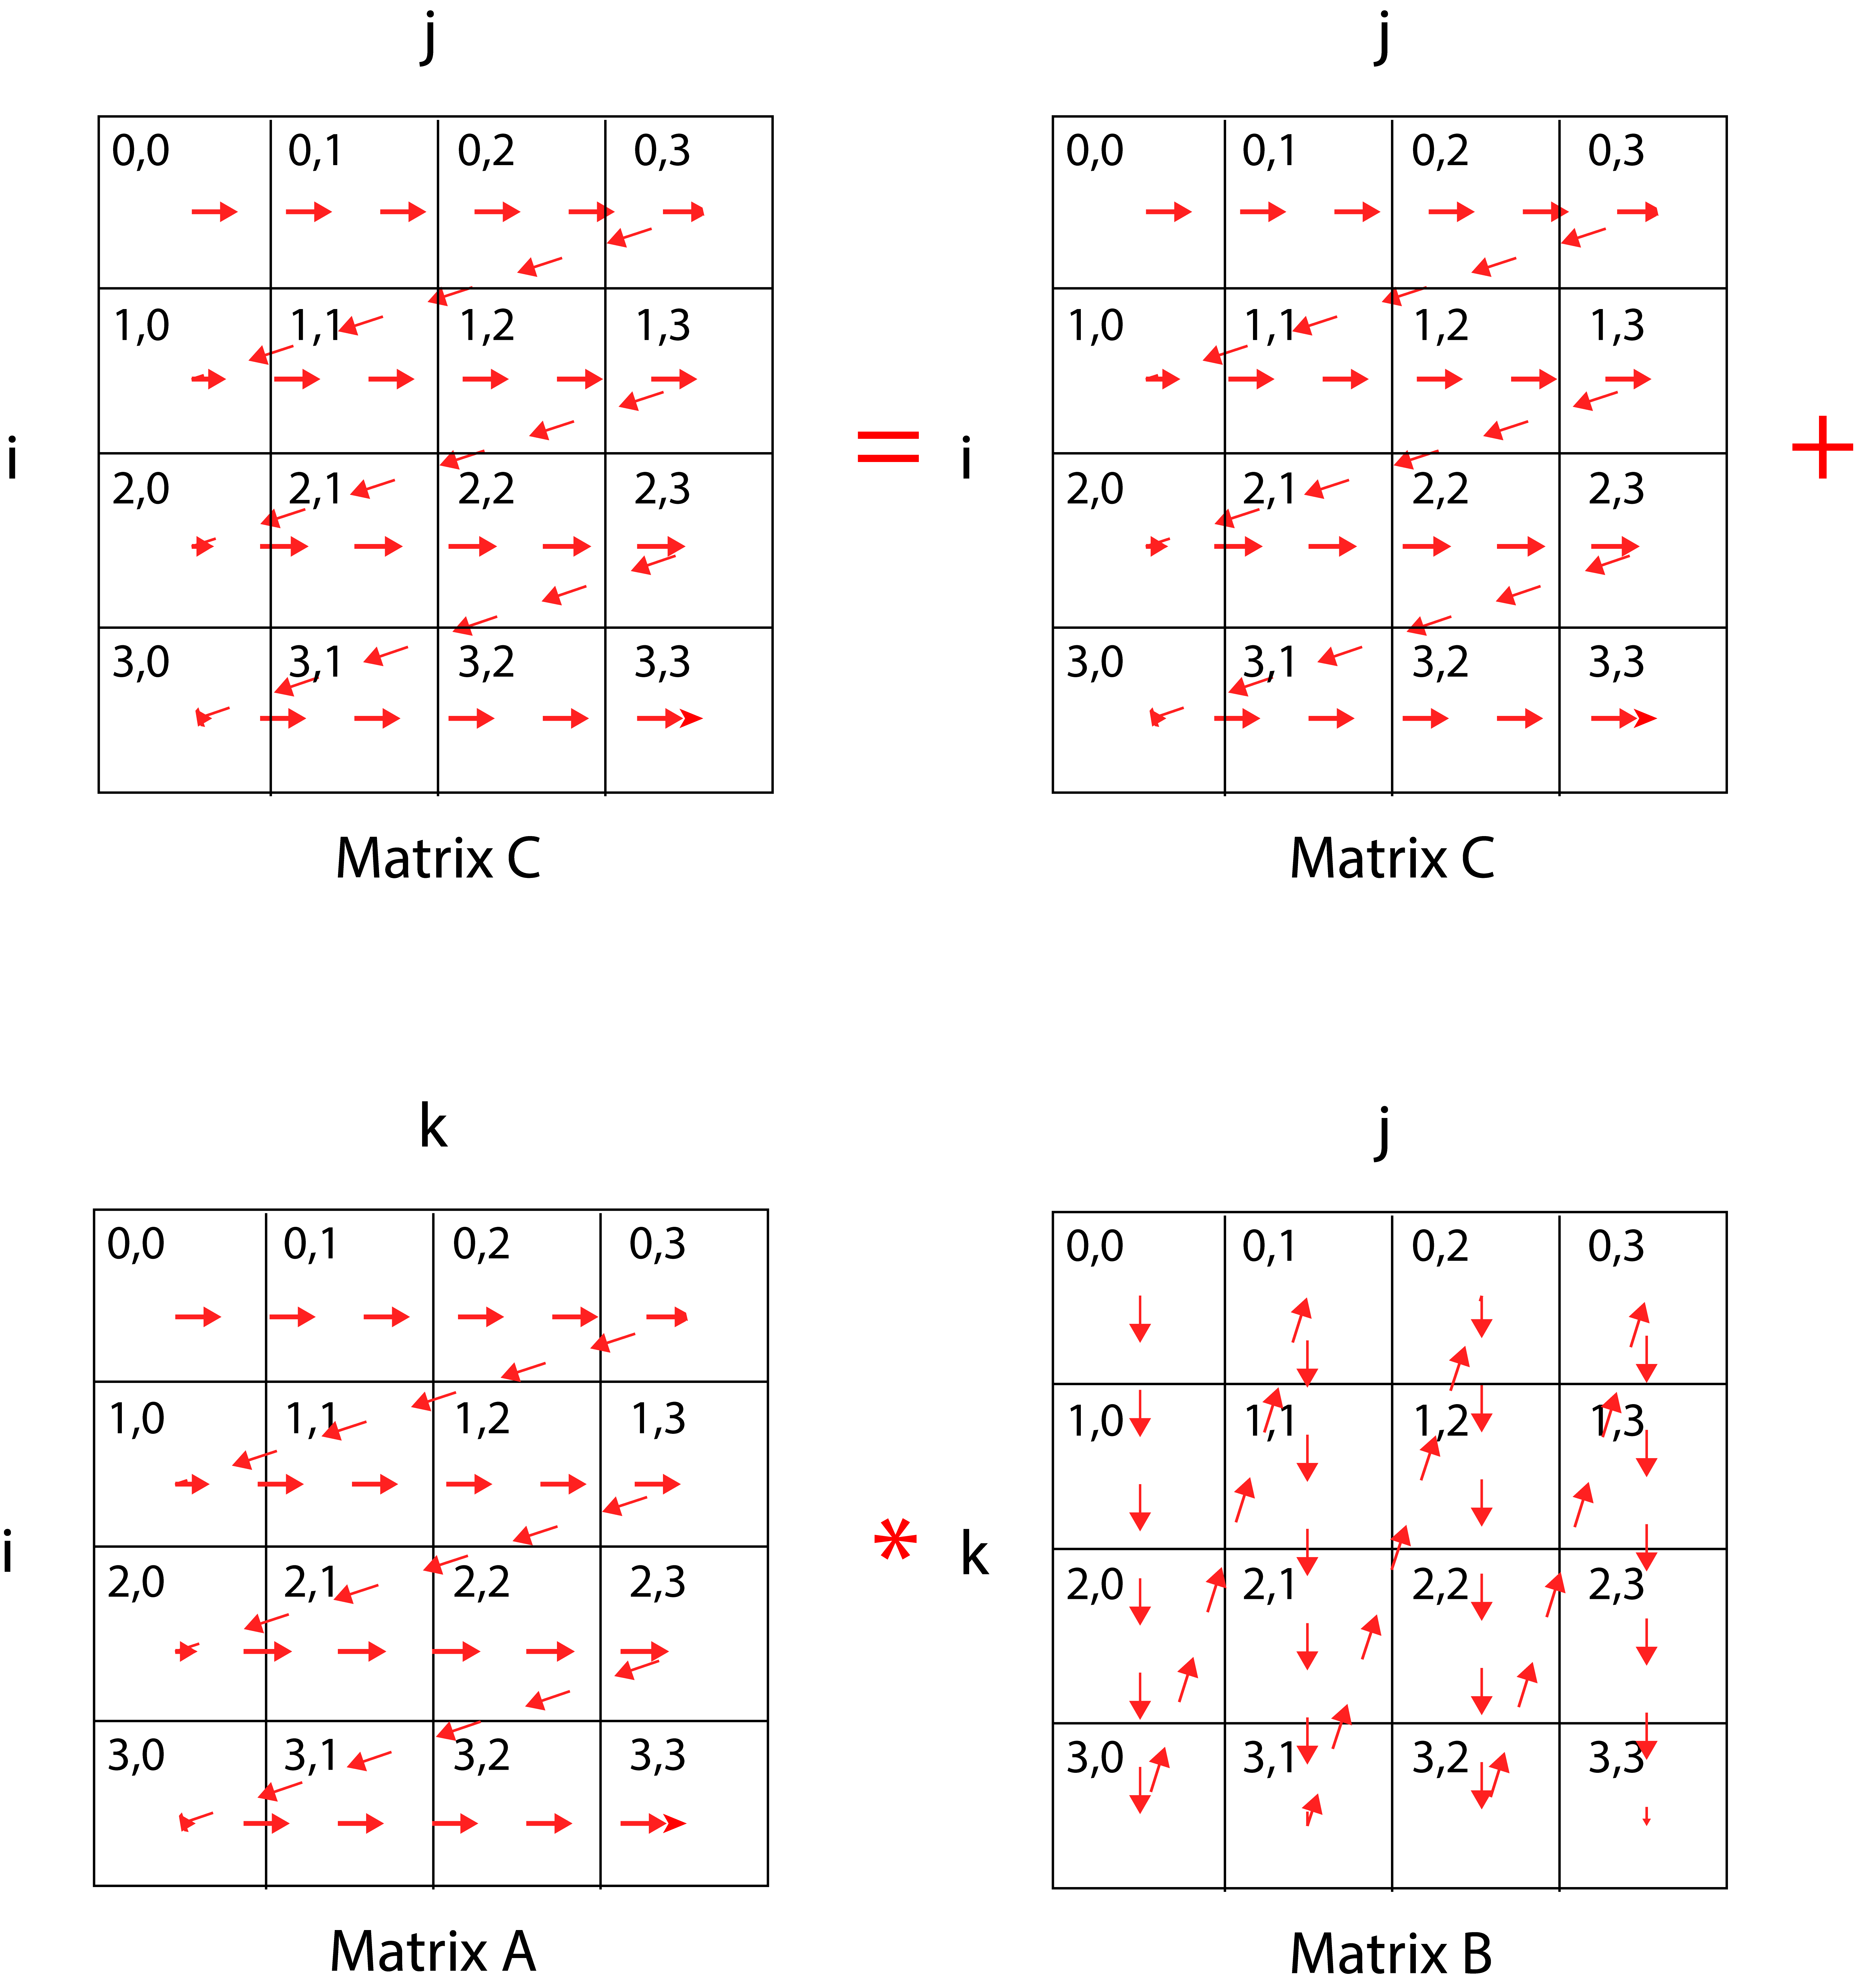
\includegraphics[width=0.9\columnwidth]{images/matrix_ijk_final.png}
\caption{Visual loop cycles evolution in nested loops order ijk}
\label{figure:loop_ijk}
\end{figure}

On each iteration, the value of k is incremented. Therefore each iteration of the innermost loop is likely to produce a cache miss loading the value of B[k][j]. That is due to matrix B being stored in row major order, resulting in an access pattern to the values of matrix B with a stride of N.\par 

\subsection{Nested Loops for single threaded dot ikj}

Given the defined matrices and their size, considering the loop order ikj, we compute their product based on the function in the appendix \ref{appendix:mm_ikj.c}.

For the specific nested loops order, all matrices are accessed row major, as described in figure \ref{figure:loop_ikj}.

\begin{figure}[H]
\centering
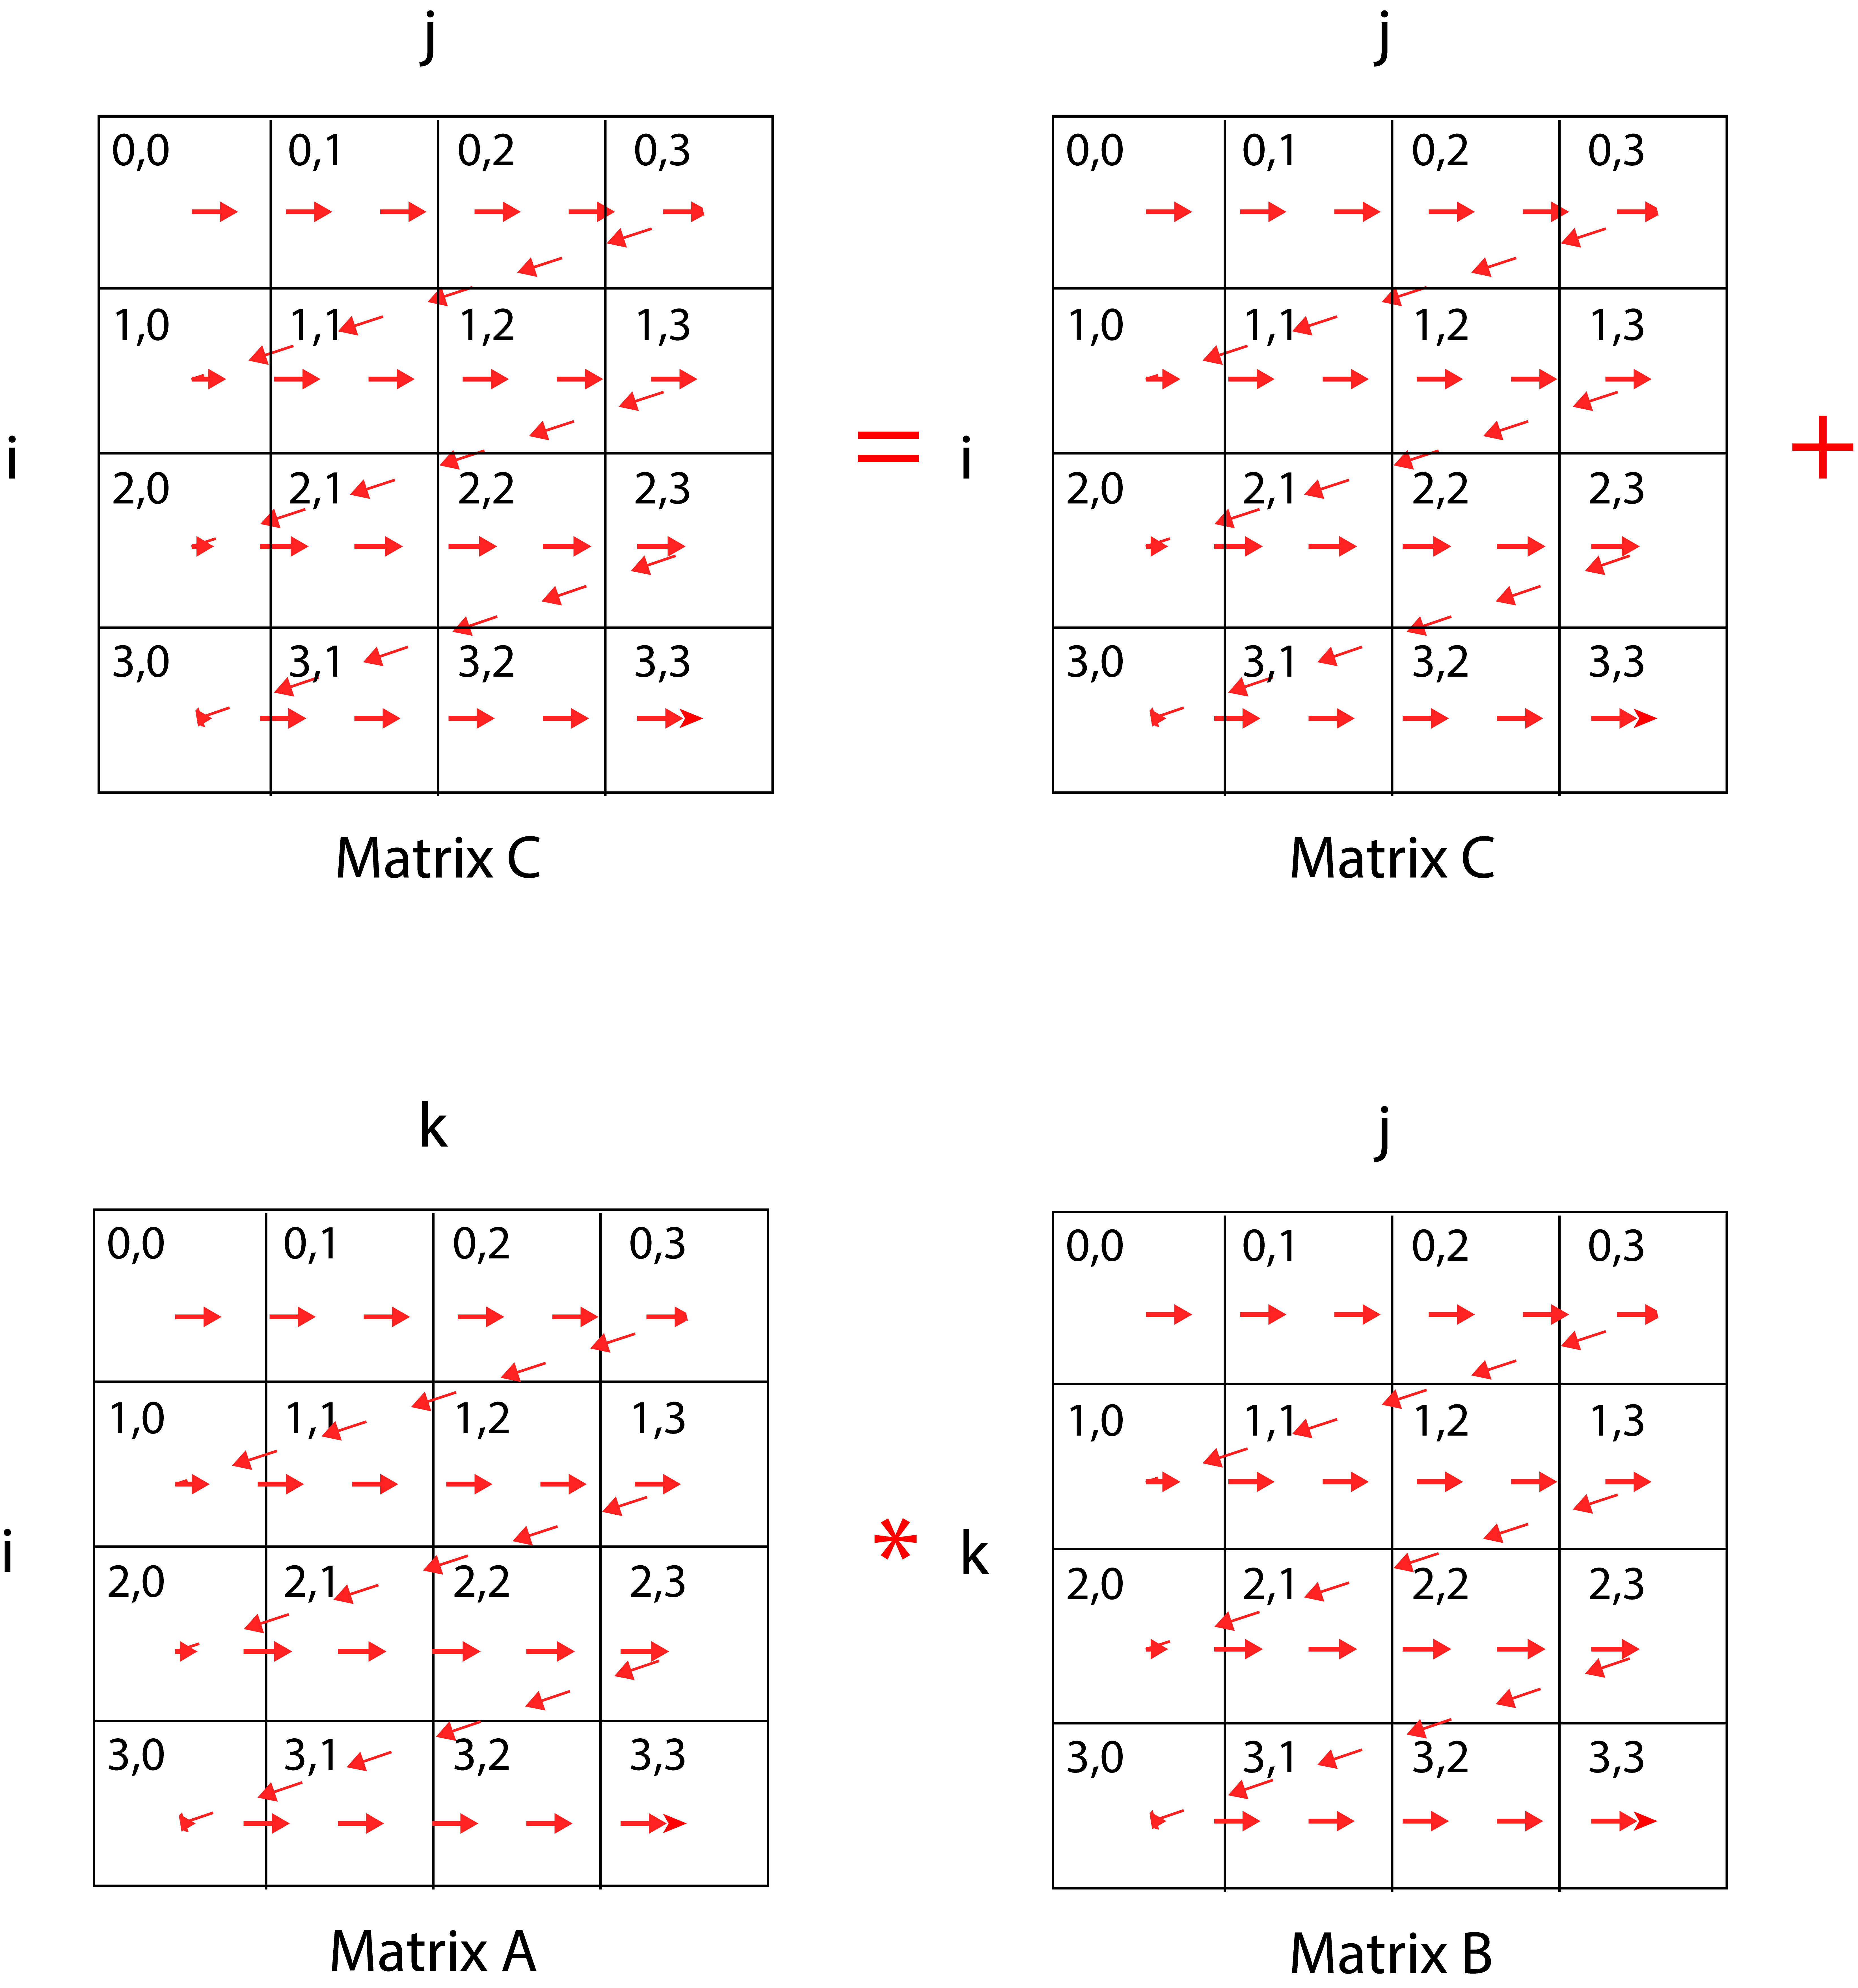
\includegraphics[width=0.9\columnwidth]{images/matrix_ikj_final.png}
\caption{Visual loop cycles evolution in nested loops order ikj}
\label{figure:loop_ikj}
\end{figure}

Note that the nesting of the innermost loops
has been changed. The index variables j and k
change the most frequently and the access
pattern through the operand matrices is
sequential using a small stride (one). This
change improves access to memory data through
the data caches. 



\subsection{Algorithm Validation}
After the development of the algorithm, we proceed to its validation. For that we fill a square matrix A [Table \ref{table:A}] with randomly generated values and a matrix B [Table \ref{table:B}] where all elements are "1" Like we can see in appendix \ref{appendix:algValA} and appendix \ref{appendix:algValB} respectively. Given the A and B matrices we execute the code and obtain a C [Table \ref{table:AB}] matrix corresponding to the dot product A*B. The result can be consulted on Appendix \ref{appendix:algValAB}.Note that all elements from a line present the same value for matrix C.\par 
Given the same A and B matrices we then produce a C [Table \ref{table:BA}] matrix corresponding to the dot product B*A. The result can be consulted on Appendix \ref{appendix:algValBA}. Note that all elements from a column present the same value for matrix C.


\subsection{Getting the best execution time for IJK and IKJ kernels}

Based on the earlier describe PAPI  (PAPI\_get\_real\_usec()) the best execution time was acquired and is related to matriz side size in the following table: 

\begin{table}[H]
\centering
  \begin{tabular}{ | L{1.5cm} | R{1.5cm} | R{1.5cm} |R{2cm} | }
      \hline

Matrix size	&IJK  ($\mu$s)&	IKJ ($\mu$s)&	IKJ vs IJK \% improvement \\
    \hline
48*48 &	500	& 564	&-11.35\% \\
128*128	&10097	&9141	&10.46\% \\
512*512	&823435	&594963	&38.40\% \\
2048*2048	&114944461	&36889436&	211.59\% \\
    \hline

\end{tabular}
\caption{Relation between matrices side size, kernel and execution time}
\label{table:table_mem}
\end{table}


\subsection{USING PAPI counters do compose metrics}
The earlier described PAPI  counters  allowed  us  to  calculate
a number of composite metrics, including bandwidth usage,
floating point instructions per second, ram accesses rates and operational intensity. Each of the following composite metrics are presented in the following tables.



\subsubsection{Total Bytes transferred to/from RAM}


\begin{table}[H]
\centering
  \begin{tabular}{ | L{1.5cm} | R{1.8cm} |  R{1.8cm} | R{1.8cm} |}
    \hline
&	IJK	 &	IKJ &\\
    \hline

Matrix side size &	Total Read Write Bytes	&	Total Read Write Bytes	&	Improvement Factor \\
    \hline

48*48	& 11,938	KB	&13,438	KB	&-0,11 \\
128*128	&82,875	KB	&24,500	KB	&2,38\\
512*512	&5,026	MB	&1,433	MB	&2,51\\
2048*2048	&32,718	GB	&1,460	GB	&21,40\\
			\hline
\end{tabular}
\caption{Relation between matrix side size, kernel, and total read/write bytes RAM.}
\label{table:vector}
\end{table}	



\begin{table}[H]
\centering
  \begin{tabular}{ | L{1.5cm} | R{3cm} | R{2cm} |}
    \hline
   \multicolumn{3}{|c|}{IJK}  \\
    \hline
Matrix side size &	Total FP Operations & 	GFlops/s \\
    \hline
48*48&	1115188&	2,226\\
128*128	&21882174&	2,119\\
512*512	&2637729392&	3,178\\
2048*2048&	198096827725&	1,728\\
			\hline
\end{tabular}
\caption{Relation between matrix side size, total FP Operations and GFLOPS/s,  for matrices IJK.}
\label{table:gflops_ikj}
\end{table}	
				
\begin{table}[H]
\centering
  \begin{tabular}{ | L{1.5cm} | R{3cm} | R{2cm} |}
    \hline
   \multicolumn{3}{|c|}{IKJ}  \\
    \hline
Matrix side size &	Total FP Operations & 	GFlops/s \\
    \hline
48*48&	1116696	&2,160\\
128*128&	21271101&	2,325\\
512*512&	1363894450&	2,306\\
2048*2048&	86777732645	&2,347\\
\hline
\end{tabular}
\caption{Relation between matrix side size, total FP Operations and GFLOPS/s,  for matrixes IKJ.}
\label{table:gflops_ikj}
\end{table}

While the kernel IKJ kept approximately the same value of Floating Point Operations computed per second for each dataset size, the kernel IJK demonstrated more unstable behavior variating between 3.178 and 1.728 GFLOPS for different dataset sizes. 

\subsubsection{L2 and L3 Cache Misses per Load}

Another important metric for application performance is the
last level cache (LLC) miss percentage. Modern CPUs rely heavily on caching to minimize the cost
of data loads and stores.
\begin{table}[H]
\centering
  \begin{tabular}{ | L{1.5cm} | R{1.2cm} | R{1.2cm} |R{1.2cm} |R{1.2cm} |  }
    \hline
   &   \multicolumn{2}{|c|}{IJK} &   \multicolumn{2}{|c|}{IKJ} \\
       \hline

Matriz Size & \% L2 C. Misses &\% L3 C. Misses & \% L2 C. Misses & \% L3 C. Misses \\
\hline
48*48 & 34,51\% & 65,33\% & 30,17\% &46,36\% \\
128*128 & 5,93\% & 10,02\% & 3,09\% & 11,58\% \\
512*512 & 5,76\% & 3,37\% & 10,82\% & 2,42\% \\
2048*2048 & 34,15\% & 10,07\% & 4,71\% & 95,2\% \\
\hline

\end{tabular}
\caption{Relation between matrix side size,L2 and L3 Cache Misses per Load.}
\label{table:table_cache}
\end{table}

Denote that he L2 and L3 Cache misses per load can lead to misleading conclusion in terms of memory dependency of the kernels.\par 
Since the percentage is based on the number of total instructions measured for the specific kernel, a smaller number of instructions from the kernel being measured may lead to a larger miss percentage. \par 


\subsubsection{RAM acesses per instruction}
As stated before we should take into account another composed metric relating also the number of total instructions and the number of total RAM accesses. 

\begin{table}[H]
\centering
  \begin{tabular}{ | L{1.5cm} | R{2.1cm} | R{2.1cm} |  R{1.5cm} | }
    \hline
   \multicolumn{4}{|c|}{IJK}  \\
	       \hline

Matrix side size&	PAPI\_LD\_INS	&PAPI\_FP\_INS&	Ram Accesses per Instruction \\
    \hline

48*48&	2445363&	223077&	11,0 \\
128*128&	46211971&	4388403&	10,5 \\
512*512	&2954122881&	527190048&	5,6 \\ 
2048*2048&	189003526449&	38091041970	&5,0 \\
\hline
\end{tabular}
\caption{Estimated Ram Accesses per instruction for kernel IJK.}
\label{table:table_cache}
\end{table}


\begin{table}[H]
\centering
  \begin{tabular}{ | L{1.5cm} | R{2.1cm} | R{2.1cm} |  R{1.5cm} | }
    \hline
   \multicolumn{4}{|c|}{IKJ}  \\
	       \hline

Matrix side size&	PAPI\_LD\_INS	&PAPI\_FP\_INS&	Ram Accesses per Instruction \\
    \hline
48*48&	2445365&	223306&	11,0 \\
128*128&	46220853&	4261260	&10,8\\
512*512&	2954125087&	272707891&	10,8\\
2048*2048&	189001037213&	17356566323	&10,9\\
\hline
\end{tabular}
\caption{Estimated Ram Accesses per instruction for kernel IKJ.}
\label{table:table_cache}
\end{table}

As shown in the precedent tables the kernel IKJ maintains the same approximate number of RAM accesses per instruction. The kernel IJK, due to the necessity of performing more loads from main memory its more unstable in terms of RAM accesses per instruction.

\subsubsection{Roofline model and the experiment results for the implemented dense squared
matrix internal product}

\begin{figure}
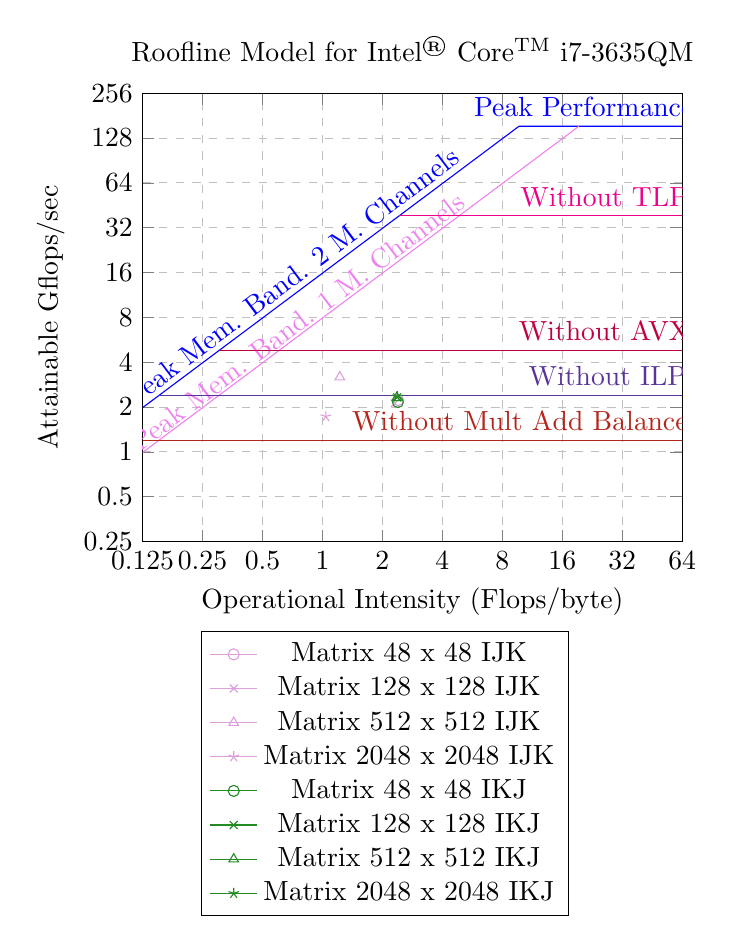
\begin{tikzpicture}

\begin{axis}[
    title={Roofline Model for Intel\textsuperscript{\textregistered} Core\textsuperscript{TM} i7-3635QM},
    xlabel={Operational Intensity (Flops/byte)},
    ylabel={Attainable Gflops/sec},
    xmin=0.125, xmax=64,
    ymin=0.25, ymax=256,
    xtick={0.125,0.25,0.5,1,2,4,8,16,32,64},
    ytick={0.25,0.5,1,2,4,8,16,32,64,128,256},
    legend style={at={(0.79,-0.2)},anchor=north east},
    ymajorgrids=true,
    xmajorgrids=true,
    grid style=dashed,
    xmode=log,
    ymode=log,
    log ticks with fixed point
]

\addplot[
    color=Plum,mark=o,
    ]
    %IJK 48*48
    coordinates{
    (2.3956,2.226)
    };
    
\addplot[
    color=Plum,mark=x,
    ]
        %IJK 128*128
    coordinates{
    (2.3051,2.119)
    };
    
\addplot[
    color=Plum,mark=triangle,
    ]
    %IJK 512*512
    coordinates{
    (1.2219,3.178)
    };
 
 \addplot[
    color=Plum,mark=star,
    ]
     %IJK 2048*2048
    coordinates{
    (1.0409,1.728)
    };
    
\addplot[
    color=ForestGreen,mark=o,
    ]
        %IJK 48*48
    coordinates{
    (2.3923,2.160)
    };
    
\addplot[
    color=ForestGreen,mark=x,
    ]
    %IKJ 128*128
    coordinates{
    (2.3717,2.325)
    };
    
\addplot[
    color=ForestGreen,mark=triangle,
    ]
    %512*512
    coordinates{
    (2.3631,2.306)
    };
    
\addplot[
    color=ForestGreen,mark=star,
    ]
    coordinates{
    (2.3761,2.347)
    };
    
 
\addplot[
    color=blue,
    ]
    coordinates {
    (0.125,1.9805)(9.695,153.6)(64,153.6)
    };
    \node[rotate=37,text=blue] at (axis cs: 0.70,15) {Peak Mem. Band. 2 M. Channels};
    
\addplot[
    color=Violet,
    ]
    coordinates {
    (0.125,0.99025)(19.389,153.6)
    };
    \node[rotate=37, text=Violet] at (axis cs: 0.75,7.5) {Peak Mem. Band. 1 M. Channels};    
    
\node [above,text=blue] at (axis cs: 20.5,153.6) {Peak Performance};
\addplot[
    color=BrickRed,
    ]
    coordinates{
    (0.07575,1.2)(64,1.2)
    };
\node [above,text=BrickRed] at (axis cs: 10.7,1.2) { Without Mult Add Balanced};

\addplot[
    color=purple,
    ]
    coordinates{
    (0.303,4.8)(64,4.8)
    };
    
\node [above,text=purple] at (axis cs: 26,4.8) { Without AVX };

\addplot[
    color=RoyalPurple,
    ]
    coordinates {
    (0.151,2.4)(64,2.4)
    };
    
\node [above, text=RoyalPurple] at (axis cs: 27,2.4) { Without ILP };

\addplot[
    color=magenta,
    ]
    coordinates {
    (2.42,38.4)(64,38.4)
    };
    
\node [above, text=magenta] at (axis cs: 26,38.4) { Without TLP };


    
     \legend{Matrix 48 x 48 IJK, Matrix 128 x 128 IJK,  Matrix 512 x 512 IJK, Matrix 2048 x 2048 IJK, Matrix 48 x 48 IKJ, Matrix 128 x 128 IKJ, Matrix 512 x 512 IKJ, Matrix 2048 x 2048 IKJ}

\end{axis}
\end{tikzpicture}
\caption{Roofline model and the experiment results for the implemented dense squared
matrix internal product.}
\label{fig:roofline_team_points}

\end{figure}

As expected the values from the experimental results for the different dataset sizes are distribute below the AVX line in Graph \ref{fig:roofline_team_points}. We should, therefore, evaluate the vectorization affectance in the algorithm performance.


\section{Vectorising the code}
Please Notice 2 different samples for IKJ kernel experiments.
Notice the following table \ref{table:no_vector}:

\begin{table}[H]
\centering
  \begin{tabular}{ | L{1.5cm} | R{2cm} |  R{3cm} | }
    \hline
Matrix side size &	PAPI\_VEC\_SP	&Total Instructions\\
    \hline
48*48 &	0&	669938\\
128*128	&0&	12761593\\
512*512&	0&	818337396\\
2048*2048&	0&	52066810629\\
			\hline
\end{tabular}
\caption{Relation between matrix side size, total FP Operations  and PAPI\_VEC\_SP.}
\label{table:no_vector}
\end{table}	

As you can see by inspecting PAPI\_VEC\_SP colum no single precision vector operation was used in the kernel.\par 
Consult the following table \ref{table:vector}:

\begin{table}[H]
\centering
  \begin{tabular}{ | L{1.5cm} | R{1.8cm}  | R{1.8cm} |}
    \hline
Matrix Side Size &	PAPI\_VEC\_SP&	PAPI\_FP\_OPS \\
    \hline
48*48 & 229448 &	1376700&
			\hline
\end{tabular}
\caption{Relation between matrix side size, total FP Operations  and PAPI\_VEC\_SP.}
\end{table}	
Please inspect PAPI\_VEC\_SP colum again.
As observed, we now have floating point vector operations in our kernel.

\subsection{Running operational intensity study for vectorized matrix IKJ of side size 48}

We will run all experiments on the platform earlier described as team laptop with equivalent measuring conditions.\par 
Given the dataset with the matrix side size of 48 the resultant test values are expressed next and compared with the non vectorized kernel.

\begin{table}[H]
\centering
  \begin{tabular}{ | L{2.5cm} | R{1.5cm} |  R{1.5cm} |  R{1.2cm} | }
    \hline
Metric &	vectorized results & non vectorized results & vectorization improvement \\
    \hline
best execution time ($\mu$s) &  73 &	564 & 6.726	\\
    \hline
\# RAM accesses per instruction  & 0,78 & 11,0	& 13.10	\\
    \hline

\# bytes transfered from/to RAM   & 22,875	KB & 13,438 KB 	&	-0.412 \\
    \hline
\# FP operations executed (GFLOPS/s)  & 26,239  &	2.160 &	11.147\\
    \hline
\# CACHE L2 miss rate &43,78\%  &  30.17\%&	-0.31\\
    \hline
\# CACHE L3 miss rate  &4,74\% &  46.36\% &	 8.78	\\

			\hline
\end{tabular}
\caption{Relation between vectorized and no vectorized kernel for IKJ dense matrix dot product.}
\label{table:vector}
\end{table}	

\subsection{Roofline Model for kernel IKJ vectorized for all datasets}

In order to predict the kernel behavior we must test all the dataset sizes.  The obtained results show the kernel reaching the TLP ceiling for almost every dataset.

\begin{figure}[H]
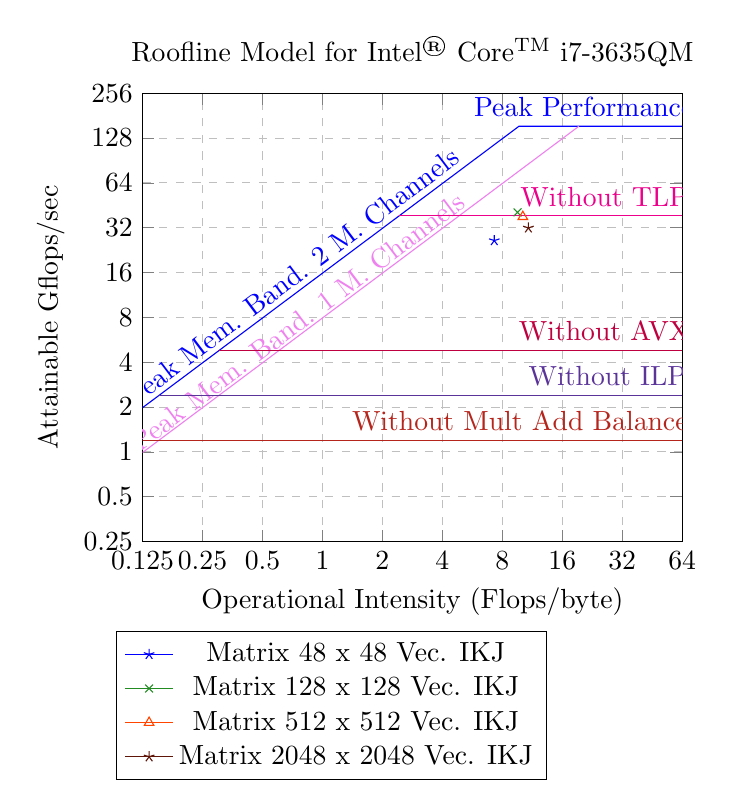
\begin{tikzpicture}
\begin{axis}[
    title={Roofline Model for Intel\textsuperscript{\textregistered} Core\textsuperscript{TM} i7-3635QM},
    xlabel={Operational Intensity (Flops/byte)},
    ylabel={Attainable Gflops/sec},
    xmin=0.125, xmax=64,
    ymin=0.25, ymax=256,
    xtick={0.125,0.25,0.5,1,2,4,8,16,32,64},
    ytick={0.25,0.5,1,2,4,8,16,32,64,128,256},
    legend style={at={(0.75,-0.2)},anchor=north east},
    ymajorgrids=true,
    xmajorgrids=true,
    grid style=dashed,
    xmode=log,
    ymode=log,
    log ticks with fixed point
]

\addplot[
    color=blue,mark=star,
    ]
    % 48*48
    coordinates{
    (7.2910,26.2394)
    };
    
    \addplot[
    color=ForestGreen,mark=x,
    ]
    % 128*128
    coordinates{
    (9.543323757,40.5768)
    };
    
\addplot[
    color=OrangeRed,mark=triangle,
    ]
    %512*512
    coordinates{
    (10.1392,37.9087)
    };
    
\addplot[
    color=Sepia,mark=star,
    ]
    %2048 2048
    coordinates{
    (10.8147,31.9131)
    };
 
 
\addplot[
    color=blue,
    ]
    coordinates {
    (0.125,1.9805)(9.695,153.6)(64,153.6)
    };
    \node[rotate=37,text=blue] at (axis cs: 0.70,15) {Peak Mem. Band. 2 M. Channels};
    
\addplot[
    color=Violet,
    ]
    coordinates {
    (0.125,0.99025)(19.389,153.6)
    };
    \node[rotate=37, text=Violet] at (axis cs: 0.75,7.5) {Peak Mem. Band. 1 M. Channels};    
    
\node [above,text=blue] at (axis cs: 20.5,153.6) {Peak Performance};
    
\addplot[
    color=BrickRed,
    ]
    coordinates{
    (0.07575,1.2)(64,1.2)
    };
\node [above,text=BrickRed] at (axis cs: 10.7,1.2) { Without Mult Add Balanced};

\addplot[
    color=purple,
    ]
    coordinates{
    (0.303,4.8)(64,4.8)
    };
    
\node [above,text=purple] at (axis cs: 26,4.8) { Without AVX };

\addplot[
    color=RoyalPurple,
    ]
    coordinates {
    (0.151,2.4)(64,2.4)
    };
    
\node [above, text=RoyalPurple] at (axis cs: 27,2.4) { Without ILP };

\addplot[
    color=magenta,
    ]
    coordinates {
    (2.42,38.4)(64,38.4)
    };
    
\node [above, text=magenta] at (axis cs: 26,38.4) { Without TLP };


    
    \legend{ Matrix 48 x 48 Vec. IKJ, Matrix 128 x 128 Vec.  IKJ, Matrix 512 x 512 Vec. IKJ, Matrix 2048 x 2048 Vec. IKJ}

\end{axis}
\end{tikzpicture}
\caption{Roofline Model for kernel IKJ vectorized}
\label{figure:roofline_vetor_points}
\end{figure}

\section{Conclusions about operational intensity}
As observed, throughput of the invocations can be bound by either the
bandwidth of the link between the core and the main memory or the throughput of the core. \par 
As observed through roofline model, for kernel IJK the greater the data set, the more memory depend will be the kernel in terms of operations.
\par The non-vectorized Kernel IKJ has maintained the approximate same performance for every type of tested dataset.\par
We can infer large scalability problems for the non-vectorized kernel IJK than for the non-vectorized kernel IKJ. \par 
The vectorized IKJ kernel as stated in Graph \ref{figure:roofline_vetor_points} is CPU bound achieving almost the peak TLP ceiling. We should, therefore, evaluate the possible TLP implementation of the algorithm in order to decrease its computing capacity limitation.\par 
TLP, which is attractive for modern multicore architectures could be achieved by inserting OpenMP directives into the kernels -- more precisely into loop templates. \par However we should take into account the overhead of thread synchronisation and all memory sharing associated problems such as false sharing.

\section{Results and Discussions}

The  roofline  model   can  help  with
identifying  effects  and  bottlenecks  due  to  memory  traffic, and
the notions of memory and compute bound are made precise and graphically visible.\par 
In therms of experimental theory validation, what  initially seemed simple tasks to execute, were extremely difficult due to several dellays based on the implementation system details and its compatibility with PAPI tool.
The source code accompanying this work assignment is available
at \cite{source}.

\newpage
\newpage
\appendix

\section{Measuring Main Memory Bandwidth}
\label{appendix:stream}
\subsection{Measuring Main Memory Bandwidth for Team's Laptop}


\lstinputlisting{code/results_personal.txt}

\subsection{Measuring Main Memory Bandwith for Search Node compute-401}

\lstinputlisting{code/cluster_results.txt}

\section{Available PAPI preset events}
For PAPI version 5.3.2, CPU Model Intel\textsuperscript{\textregistered} Core\textsuperscript{TM} i7-3635QM, operating system Ubuntu release 15.10 (wily) and kernel version 4.2.0-19-generic the following metrics were available.  
\label{appendix:papi_avail}
\begin{table}[H]
\centering
  \begin{tabular}{ | L{2.2cm} | R{6cm} |  }
      \hline
Name& Description \\
    \hline
PAPI\_L1\_DCM &  Level 1 data cache misses     \\                     
PAPI\_L1\_ICM &  Level 1 instruction cache misses   \\                       
PAPI\_L2\_DCM & Level 2 data cache misses     \\                      
PAPI\_L2\_ICM &  Level 2 instruction cache misses  \\                        
PAPI\_L1\_TCM & Level 1 cache misses   \\                         
PAPI\_L2\_TCM &  Level 2 cache misses       \\                    
PAPI\_L3\_TCM &  Level 3 cache misses    \\                     
PAPI\_TLB\_DM & Data translation lookaside buffer misses \\      
PAPI\_TLB\_IM &  Instruction translation lookaside buffer misses \\
PAPI\_L1\_LDM &  Level 1 load misses   \\                        
PAPI\_L1\_STM &  Level 1 store misses    \\                       
PAPI\_L2\_STM &  Level 2 store misses   \\                        
PAPI\_STL\_ICY & Cycles with no instruction issue  \\           
PAPI\_BR\_UCN & Unconditional branch instructions   \\          
PAPI\_BR\_CN  &  Conditional branch instructions   \\           
PAPI\_BR\_TKN & Conditional branch instructions taken     \\                       
PAPI\_BR\_NTK &  Conditional branch instructions not taken   \\                       
PAPI\_BR\_MSP &  Conditional branch instructions mispredicted  \\                         
PAPI\_BR\_PRC & Conditional branch instructions correctly predicted                          \\ 
PAPI\_TOT\_INS & Instructions completed         \\                     
PAPI\_FP\_INS & Floating point instructions     \\                        
PAPI\_LD\_INS &  Load instructions            \\                 
PAPI\_SR\_INS  & Store instructions        \\                     
PAPI\_BR\_INS &  Branch instructions        \\                     
PAPI\_TOT\_CYC & Total cycles               \\               
PAPI\_L2\_DCH & Level 2 data cache hits        \\                   
PAPI\_L2\_DCA &  Level 2 data cache accesses     \\                     
PAPI\_L3\_DCA & Level 3 data cache accesses       \\                    
PAPI\_L2\_DCR  & Level 2 data cache reads  \\                        
PAPI\_L3\_DCR &  Level 3 data cache reads    \\                      
PAPI\_L2\_DCW &  Level 2 data cache writes    \\                      
PAPI\_L3\_DCW &  Level 3 data cache writes     \\                     
PAPI\_L2\_ICH &  Level 2 instruction cache hits     \\                     
PAPI\_L2\_ICA &  Level 2 instruction cache accesses   \\                       
PAPI\_L3\_ICA &  Level 3 instruction cache accesses   \\                       
PAPI\_L2\_ICR &  Level 2 instruction cache reads   \\                       
PAPI\_L3\_ICR &  Level 3 instruction cache reads      \\                    
PAPI\_L2\_TCA & Level 2 total cache accesses    \\                       
PAPI\_L3\_TCA &  Level 3 total cache accesses   \\                       
PAPI\_L2\_TCR & Level 2 total cache reads      \\                     
PAPI\_L3\_TCR & Level 3 total cache reads      \\                     
PAPI\_L2\_TCW &  Level 2 total cache writes     \\                     
PAPI\_L3\_TCW  & Level 3 total cache writes      \\                    
PAPI\_FDV\_INS & Floating point divide instructions   \\                         
PAPI\_FP\_OPS & Floating point operations          \\                   
PAPI\_SP\_OPS & Floating point operations  optimized to count scaled single precision vector operations            \\        
PAPI\_DP\_OPS & Floating point operations  optimized to count scaled double precision vector operations            \\        
PAPI\_VEC\_SP & Single precision vector/SIMD instructions    \\                        
PAPI\_VEC\_DP & Double precision vector/SIMD instructions   \\                         
PAPI\_REF\_CYC & Reference clock cycles                         \\
    \hline

\end{tabular}
\caption{Available PAPI preset events}
\label{table:metrics}
\end{table}

\section{Algorithm Validation Appendix}
\subsection{Matrix A}
\label{appendix:algValA}
\begin{table}[H]
\centering
\begin{tabular}{| L{1.5cm} | L{1,5cm} |  L{1,5cm} |  L{1,5cm} | }
\hline
0.840188 & 0.394383 & 0.783099 & 0.798440 \\
0.911647 & 0.197551 & 0.335223 & 0.768230 \\
0.277775 & 0.553970 & 0.477397 & 0.628871 \\
0.364784 & 0.513401 & 0.952230 & 0.916195 \\
\hline
\end{tabular}
\caption{Matrix A}
\label{table:A}
\end{table}

\subsection{Matrix B}
\label{appendix:algValB}
\begin{table}[H]
\centering
\begin{tabular}{ | L{1.5cm} | L{1,5cm} |  L{1,5cm} |  L{1,5cm} | }
\hline
1.000000 & 1.000000 & 1.000000 & 1.000000 \\
1.000000 & 1.000000 & 1.000000 & 1.000000 \\
1.000000 & 1.000000 & 1.000000 & 1.000000 \\
1.000000 & 1.000000 & 1.000000 & 1.000000 \\
\hline
\end{tabular}
\caption{Matrix B}
\label{table:B}
\end{table}

\subsection{C Matrix matching the dot product A*B}
\label{appendix:algValAB}
\begin{table}[H]
\centering
\begin{tabular}{| L{1.5cm} | L{1,5cm} |  L{1,5cm} |  L{1,5cm} | }
\hline
2.816110 & 2.816110 & 2.816110 & 2.816110 \\
2.212651 & 2.212651 & 2.212651 & 2.212651 \\
1.938013 & 1.938013 & 1.938013 & 1.938013 \\
2.746610 & 2.746610 & 2.746610 & 2.746610 \\
\hline
\end{tabular}
\caption{C Matrix matching the dot product A*B}
\label{table:AB}
\end{table}

\subsection{C Matrix matching the dot product B*A}
\label{appendix:algValBA}
\begin{table}[H]
\centering
\begin{tabular}{ | L{1.5cm} | L{1,5cm} |  L{1,5cm} |  L{1,5cm} | }
\hline
2.394394 & 1.659305 & 2.547949 & 3.111736 \\
2.394394 & 1.659305 & 2.547949 & 3.111736 \\
2.394394 & 1.659305 & 2.547949 & 3.111736 \\
2.394394 & 1.659305 & 2.547949 & 3.111736 \\
\hline
\end{tabular}
\caption{C Matrix matching the dot product B*A}
\label{table:BA}
\end{table}

\section{Matrix functions for each loop}
\subsection{Function for loop IJK}
\label{appendix:mm_ijk.c}
\lstinputlisting{code/mm_ijk.c}

\subsection{Function for loop IKJ}
\label{appendix:mm_ikj.c}
\lstinputlisting{code/mm_ikj.c}

% We recommend abbrvnat bibliography style.

\bibliographystyle{abbrvnat}
\bibliography{references}

\end{document}